\begin{figure}[!ht]
	\centering
	\setlength{\resLen}{.875in}
	\setlength{\raiseLen}{.1in}
	\addtolength{\tabcolsep}{-5pt}
	\vspace{-30pt}
	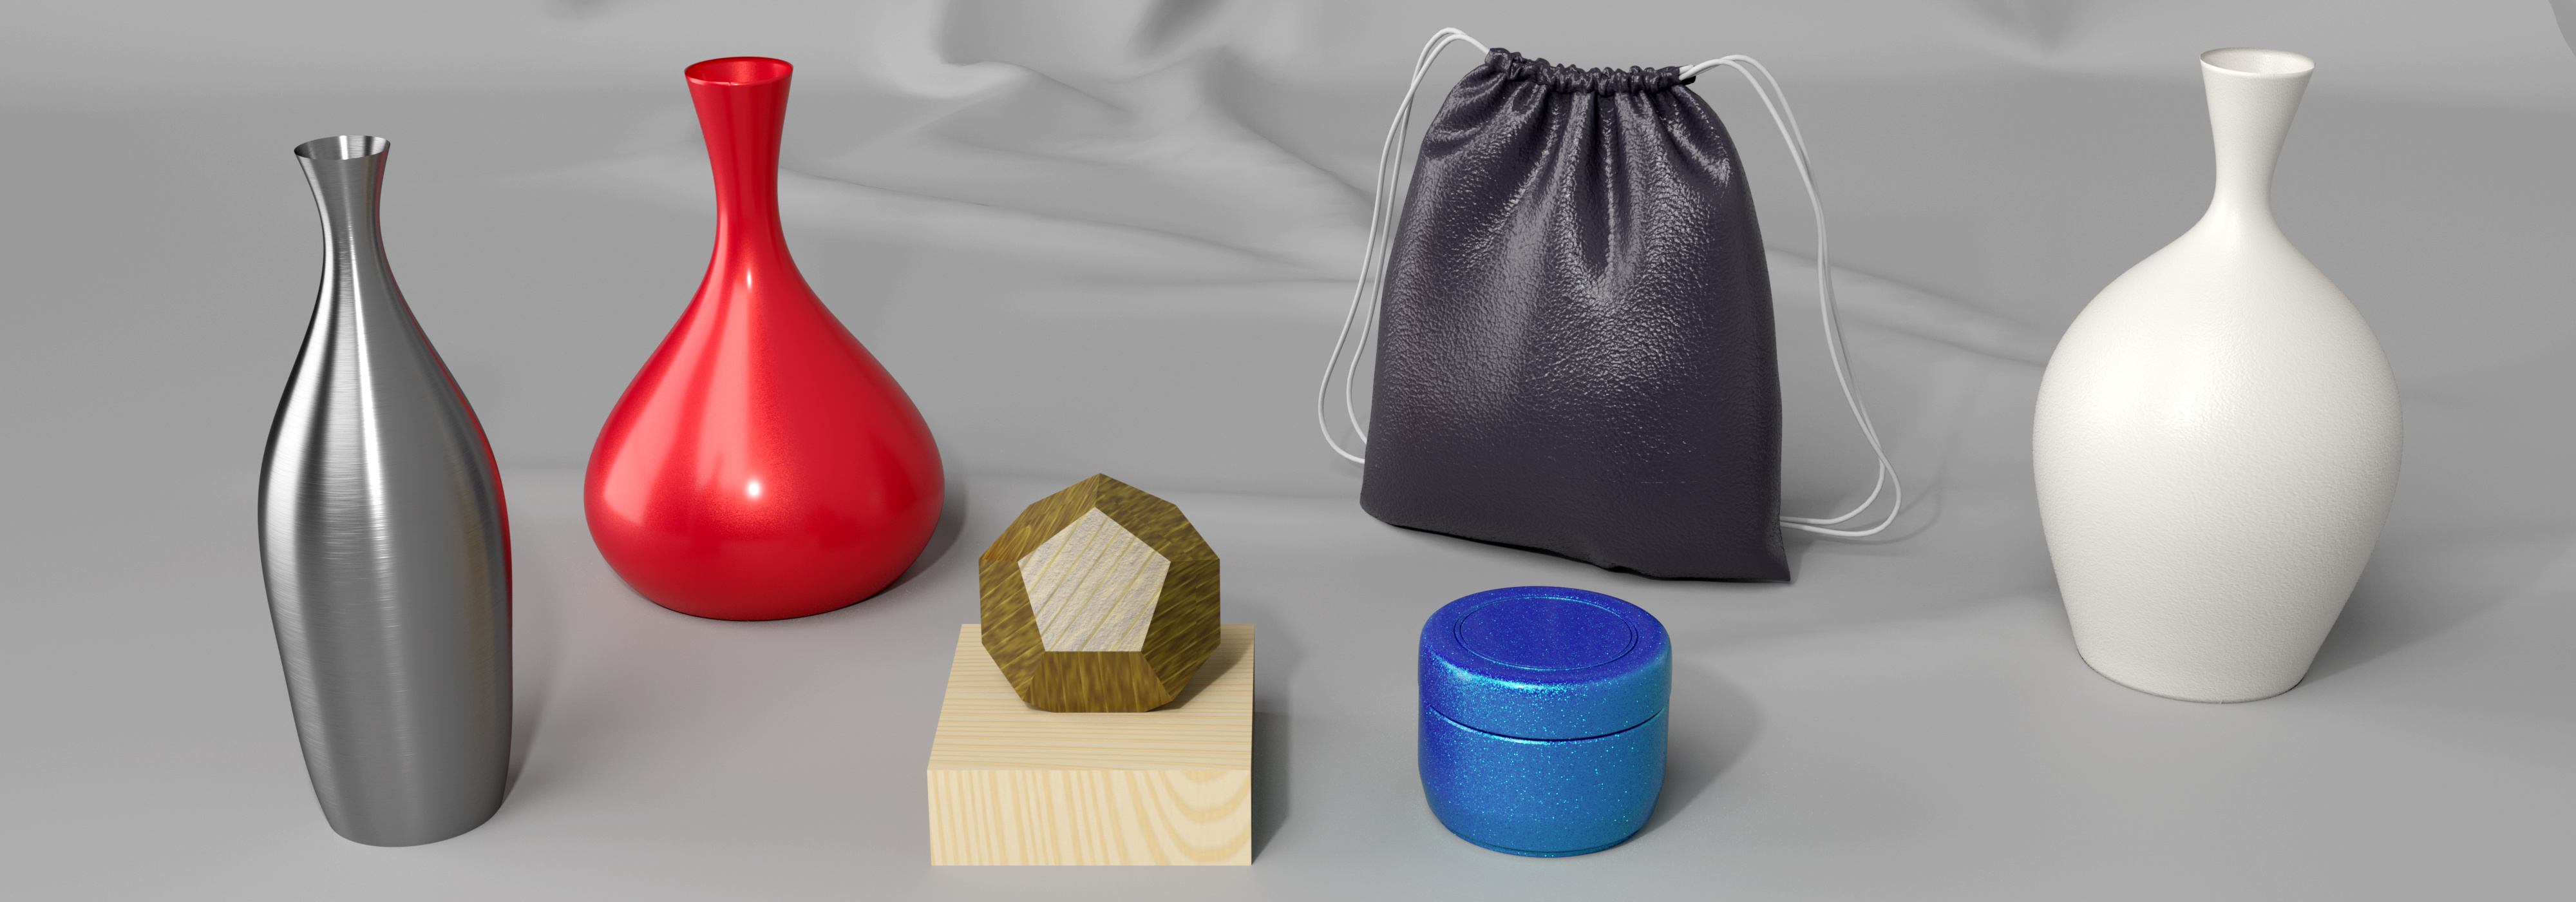
\includegraphics[width=\textwidth]{bayesian/fig1-2/teaser.jpg}\\[2pt]
	\begin{tabular}{cccccccc}
		\raisebox{\raiseLen}{\rotatebox{90}{Input}} &
		
\includegraphics[width=\resLen]{bayesian/fig7/5_metal_3/target.jpg} &
		
\includegraphics[width=\resLen]{bayesian/fig7/4_flake_4/target.jpg} &
		
\includegraphics[width=\resLen]{bayesian/fig7/6_wood_4/target.jpg} &
		
\includegraphics[width=\resLen]{bayesian/fig7/6_wood_5/target.jpg} &
		
\includegraphics[width=\resLen]{bayesian/fig5/4_flake_1/target.jpg} &
		
\includegraphics[width=\resLen]{bayesian/fig7/2_leather_3/target.jpg} &
		
\includegraphics[width=\resLen]{bayesian/fig7/1_bump_4/target.jpg}
		\\
		\raisebox{\raiseLen}{\rotatebox{90}{Rendered}} &
		\includegraphics[width=\resLen]{bayesian/fig7/5_metal_3/good1.jpg} &
		\includegraphics[width=\resLen]{bayesian/fig7/4_flake_4/good1.jpg} &
		\includegraphics[width=\resLen]{bayesian/fig7/6_wood_4/good1.jpg} &
		\includegraphics[width=\resLen]{bayesian/fig7/6_wood_5/good1.jpg} &
		\includegraphics[width=\resLen]{bayesian/fig5/4_flake_1/good1.jpg} &
		\includegraphics[width=\resLen]{bayesian/fig7/2_leather_3/good1.jpg} &
		\includegraphics[width=\resLen]{bayesian/fig7/1_bump_4/good1.jpg}
	\end{tabular}
	\caption[Teaser]{\label{fig:bayesian:teaser}
		A scene rendered with material parameters estimated using our method: bumpy dielectrics, leather, plaster, wood, brushed metal, and metallic paint. The insets show a few examples of the input (target) images, and renderings produced using our procedural models with parameters found by Bayesian posterior sampling.
 	}
\end{figure}
